%auto-ignore
\documentclass{standalone}

\usepackage{graphicx}
\usepackage{tikz}

\begin{document}
\begin{tikzpicture}
\node[inner sep=0pt,align=center]
(pamg_1) at (0,0)
	{
\includegraphics[width=.15\textwidth]{figure7_10.jpg}\\[1em]
	 
\includegraphics[width=.15\textwidth]{figure7_20.jpg}\\[1em]
	 
\includegraphics[width=.15\textwidth]{figure7_30.jpg}\\[1em]
	 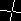
\includegraphics[width=.15\textwidth]{figure7_40.jpg}};
\node[inner sep=0pt,align=center]
(pamg_2) at (5,0)
	{
\includegraphics[width=.15\textwidth]{figure7_11.jpg}\\[1em]
	 
\includegraphics[width=.15\textwidth]{figure7_21.jpg}\\[1em]
	 
\includegraphics[width=.15\textwidth]{figure7_31.jpg}\\[1em]
	 
\includegraphics[width=.15\textwidth]{figure7_41.jpg}};
\node[inner sep=0pt,align=center]
(pamg_3) at (10,0)
	{
\includegraphics[width=.15\textwidth]{figure7_12.jpg}\\[1em]
	 
\includegraphics[width=.15\textwidth]{figure7_22.jpg}\\[1em]
	 
\includegraphics[width=.15\textwidth]{figure7_32.jpg}\\[1em]
	 
\includegraphics[width=.15\textwidth]{figure7_42.jpg}};
\node[inner sep=0pt,align=center]
(pamg_4) at (15,0)
	{
\includegraphics[width=.15\textwidth]{figure7_13.jpg}\\[1em]
	 
\includegraphics[width=.15\textwidth]{figure7_23.jpg}\\[1em]
	 
\includegraphics[width=.15\textwidth]{figure7_33.jpg}\\[1em]
	 
\includegraphics[width=.15\textwidth]{figure7_43.jpg}};
\draw[->,thick,shorten >=6pt,shorten <=6pt] (pamg_1) -- (pamg_2)
	node[midway,fill=white,align=center,rotate=90,anchor=north,yshift=0.4cm]
	{\huge dilate};
\draw[->,thick,shorten >=6pt,shorten <=6pt] (pamg_2) -- (pamg_3)
	node[midway,fill=white,align=center,rotate=90,anchor=north,yshift=0.4cm]
	{\huge border\\around};
\draw[->,thick,shorten >=6pt,shorten <=6pt] (pamg_3) -- (pamg_4)
	node[midway,fill=white,align=center,rotate=90,anchor=north,yshift=0.4cm]
	{\huge find\\rhomboids};
\end{tikzpicture}
\end{document}
\documentclass{standalone}
